\documentclass[defense.tex]{subfiles}
\begin{document}


\begin{frame}<presentation:0>{}

\centering\Huge {\color{darkred}\textbf {Part I}}:\\
Adaptive Sparse Coding\\
\biblio{}
	
\end{frame}


\section{Adaptive Iterative Soft Thresholding}
\label{sec:adapt}


\begin{frame}{LASSO}
	The LASSO or sparse coding problem searches for $z^*$ such that 
	
	\begin{equation}
        \label{eq:lasso}
        z^* = \argmin_z F(z) := \underbrace{\frac{1}{2}\|x - Dz\|_ 2^2}_{E(z)} + \lambda\|z\|_1~,
	\end{equation}
	
	where $x \in \mathbb R^P$, $D \in \mathbb R^{P\times K}$ and $z \in \mathbb R^K$.\\[2em]

	
	We denote $B = D\tran D$ is the Gram matrix of $D$.
\end{frame}

\begin{frame}{The quadratic-form $Q_S$}

	Define $Q_S(u, v) = \frac{1}{2}(u-v)\tran S (u-v) + \lambda \|u\|_1~.$\\[.5em]
	If $S$ is diagonal, the following problem can efficiently be solved:
	\[
		\argmin_u Q_S(u, v)
	\]
	\vskip1em
	The problem is separable on each coordinate:
	\[
		\argmin_{u_i}\frac{s_i}{2}(u_i - v_i)^2 + \lambda\|u_i\|
	\]
	\hskip2em $\Rightarrow$  Scaled soft thresholding
	\[
		u_i^* = \frac{\text{sign}(v_i)}{s_i}\max(0, |v_i| - \lambda)
	\]
	

	
\end{frame}



\begin{frame}[t]{Toward an adaptive procedure}
	Given an estimate $z^{(q)}$ of $z^*$ at iteration $q$, we can write:
	\begin{eqnarray*}
		F(z) & =& E(z) + \lambda\|z\|_1\\
		     & = & E(z^{(q)}) + \left\langle \nabla E(z^{(q)}) , z-z^{(q)} \right\rangle
						+ Q_{\makebox[.7em][c]{$B$}}(\phantom{\bf A}z, \phantom{\bf A}z^{(q)})~,\\
	\end{eqnarray*}%
	\vskip-1em
	\only<1>{\color{lightblue!70}}%
	\underline{\bf ISTA:} ~~~~~Replace $B$ by diagonal matrix $S = L\pmb I_K$ \\[.5em]
	\only<2>{\color{lightblue!70}}%
	\underline{\bf FacNet:} ~~Replace $B$ by $A\tran S A$ ~~~($S$ diagonal, $A$ unitary)
	\only<-2>{\color{black}}\\
	\vskip-.5em
	\begin{eqnarray*}
	\only<2>{
		F_q(z) & = & E(z^{(q)}) + \left\langle \nabla E(z^{(q)}) , z-z^{(q)} \right\rangle
						+ Q_{\makebox[.9em][c]{\color{blue!75}$\bf S_q$}}
								(\phantom{\bf A_q}z, \phantom{\bf A_q}z^{(q)})~,\\
			   \min_z F_q(z)& \Leftrightarrow & \min_z Q_{S_q}\Big(\phantom{A_q}z, \phantom{A_q}z^{(q)}
			   								    - \text{\makebox[2.5em][c]{$S_q^{-1}$}}\nabla E(z^{(q)})\Big)
	}
	\only<3-4>{
		\widetilde F_q(z) & = &
					E(z^{(q)}) + \left\langle \nabla E(z^{(q)}) , z-z^{(q)} \right\rangle
						+ Q_{\makebox[.9em][c]{$S_q$}}({\bf\color{blue!75} A_q}z, {\bf\color{blue!75} A_q}z^{(q)})~,\\
						\min_z \widetilde F_q(z)& \Leftrightarrow & \min_z Q_{S_q}\Big(A_qz, A_qz^{(q)}
						  - \text{\makebox[2.5em][c]{$S_q^{-1}A_q$}}\nabla E(z^{(q)})\Big)
	}
	\end{eqnarray*}
	\only<1-3>{\color{lightblue!70}}
	Can we choose $A_q, S_q$ to accelerate the optimization compared to ISTA?

\end{frame}

\begin{frame}{Quadratic form}
\centering
\only<1>{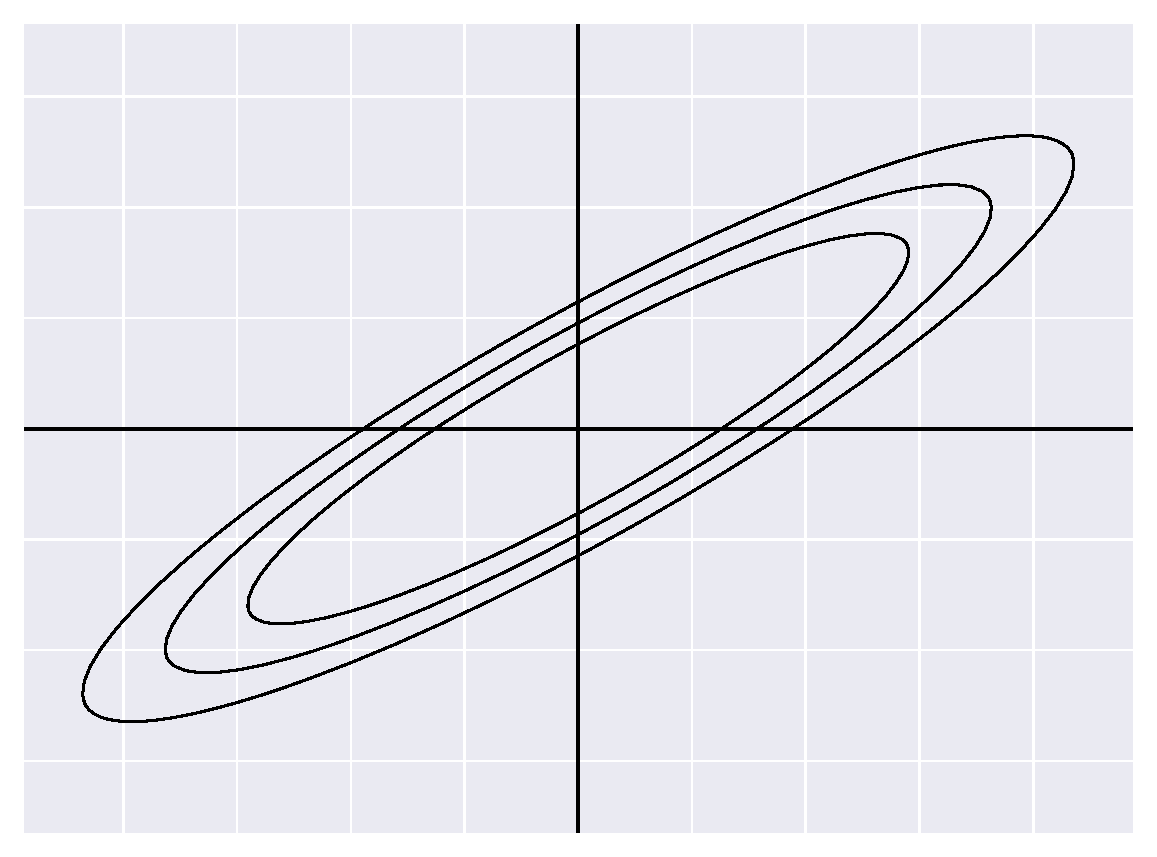
\includegraphics[height=.9\textheight]{ell1}}
\only<2>{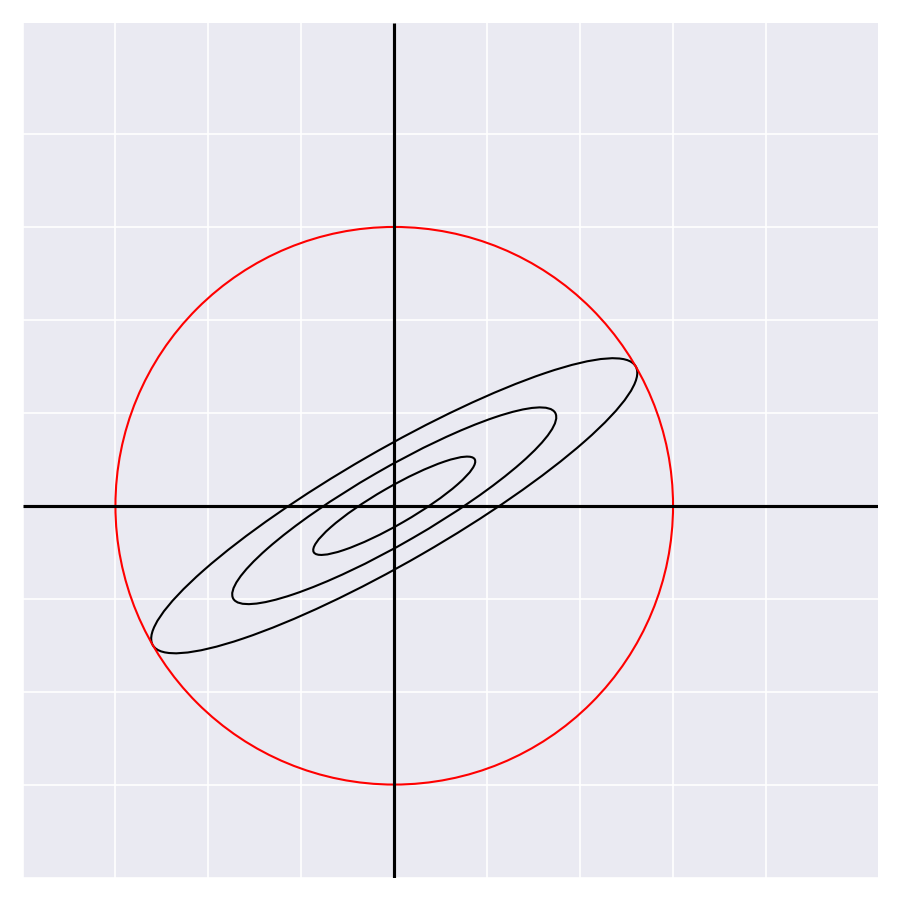
\includegraphics[height=.9\textheight]{ell2}}
\only<3>{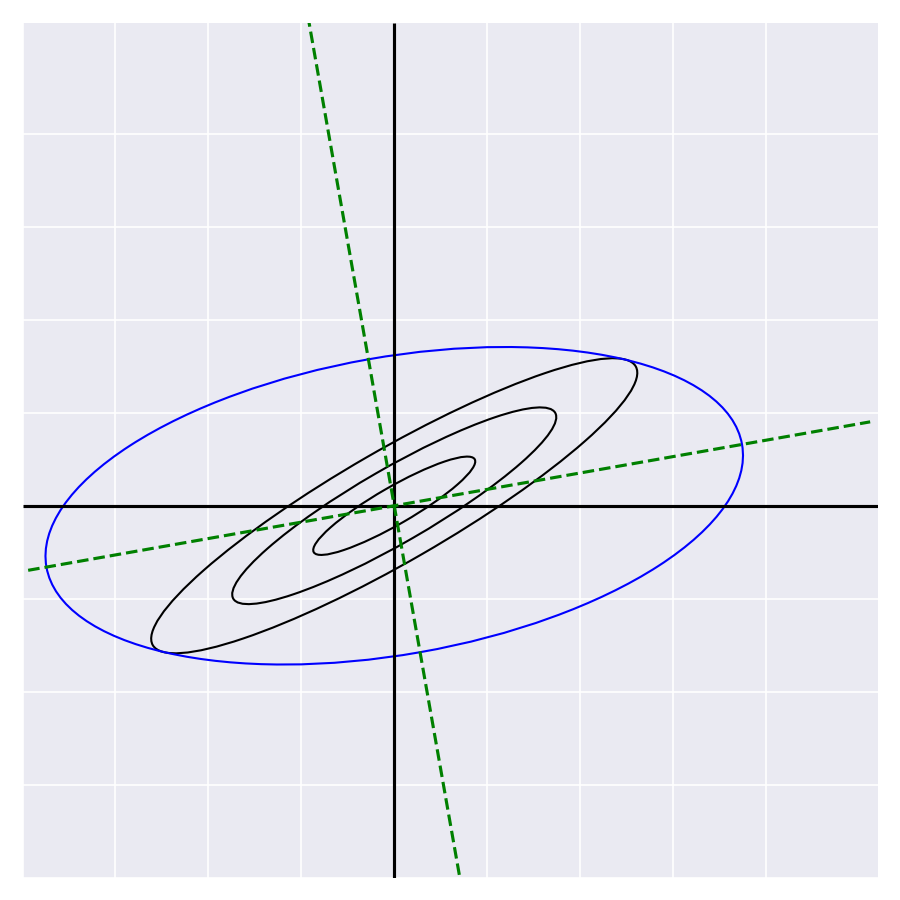
\includegraphics[height=.9\textheight]{ell3}}
	
\end{frame}

\begin{frame}{Iterative procedures}

	\textbf{ISTA:}\\
	\begin{eqnarray*}
		z^{(q+1)} & = & \argmin_z F_q(z)\\
		          & = & \prox_{S}( z^{(q)} -  \frac{1}{\|B\|_2} \nabla E(z^{(q)}))~,
	\end{eqnarray*}
	\textbf{FacNet:}\\
	\begin{eqnarray*}
		z^{(q+1)} & = & \argmin_z \widetilde F_q(z)\\
			& = & A_q\tran \prox_{S}( A_qz^{(q)} - S_q^{-1}A_q \nabla E(z^{(q)}))~,
	\end{eqnarray*}
	
\end{frame}


\begin{frame}{Toward an adaptive procedure}
	

	Similar iterative procedure with steps adapted to the problem topology.\\[1em]
	\[
		\widetilde{F_q}(z) = F(z) + (z-z^{(q)})\tran R(z-z^{(q)}) + \delta_A(z)
	\]
%\textbf{Proximal resolution :}
%\[z^{(q+1)} = \argmin_z F(z) = E(z^{(q)}) + \langle B(z^{(q)}-y) , z-z^{(q)} \rangle + \frac{1}{2}\| z - z^{(q)} \|_B^2 + G(z)~ ,\]
%$\color{darkblue}\Rightarrow$ Not computationally efficient but quick minimization.\\[1.5em]


	Tradeoff between:\\[.3em]
	\begin{itemize}\itemsep1em
		\item Rotation to align the norm $\|\cdot\|_B$ and the norm $\|\cdot\|_1$~,
		\keypoint{Computation}
		\[ R = A\tran SA - B\]
		\item Deformation of the $\ell_1$-norm with the rotation $A$~.
		\keypoint{Accuracy}
		\[ \delta_A(z) = \lambda\left(\|Az\|_1-\|z\|_1\right) \]
	\end{itemize}
	
\end{frame}


\begin{frame}{One step improvement	}
	\begin{block}{Proposition}
		\label{bi1}
		Suppose that $R_q = A_q\tran S_q A_q - B \succ 0$ is positive definite, and define 
		\[z^{(q+1)} = \arg\min_z \widetilde{F_q}(z)~,\]
		Then
		\[
			F(z^{(q+1)}) - F(z^*) \leq \frac{1}{2}(z^{(q)} - z^*)\tran R_q (z^{(q)} - z^*)
									+ \delta_{A_q}(z^*) - \delta_{A_q}(z^{(q+1)})~.
		\]
	\end{block}
	\vskip2em
	We are interested in factorization $(A_q, S_q)$ for which $\|R_q\|_2$\\and $\delta_{A_q}$  are small.
\end{frame}

\begin{frame}{Adaptive Iterative Soft thresholding - Convergence rate \mycite{Moreau2017}}

    \begin{block}{Theorem}
    Let $A_q, S_q$ be the pair of unitary and diagonal matrices corresponding to iteration $q$, 
chosen such that $R_q = A_q\tran S_q A_q - B \succ 0$.
It results that
{\small 
\begin{equation*}
\label{zo1}
%F(z_{k}) - F(z^*) \leq \frac{(z^*- z_0)\tran R_0 (z^* - z_0) + 2 |\delta_{A_0}(z_{1}) - \delta_{A_0}(z^*) | }{2k} + \frac{\alpha - \beta}{2k}~,\text{ with}
	\begin{split}
		F(z^{(q)}) - F(z^*) \leq &\frac{(z^*- z^{(0)})\tran R_0 (z^* - z^{(0)}) + 2 L_{A_0}(z^{(1)}) \|  (z^*-z^{(1)}) \|_2 }{2q}\\
			&\hskip3em + \frac{\alpha_q - \beta_q}{2q}~,
	\end{split}
\end{equation*}
%$$\alpha = \sum_{n=1}^{k-1} \left(  2| \delta_{A_n}(z_{n+1}) - \delta_{A_n}(z^*)| + (z^* - z_n)\tran ( R_{n-1} - R_{n}) (z^* - z_n) \right)~,$$
\[\alpha_q = \sum_{i=1}^{q-1} \left(  2L_{A_i}(z^{(i+1)})\|(z^*-z^{(i+1)}) \| + (z^* - z^{(i)})\tran ( R_{i-1} - R_{i}) (z^* - z^{(i)}) \right)~,\]
\[\beta_q = \sum_{i=0}^{q-1} (i+1)\left((z^{(i+1)}-z^{(i)})\tran R_i (z^{(i+1)}-z^{(i)}) + 2\delta_{A_i}(z^{(i+1)}) - 2\delta_{A_i}(z^{(i)}) \right)~,\]}
where $L_A(z)$ denote the local Lipschitz constant of $\delta_A$ at $z$.
    \end{block}
\end{frame}

\begin{frame}{Interpretation}

	\begin{itemize}\itemsep2em
		\item For $A_q = \pmb I_K$ and $S_q = \|B\|_2 \pmb I_K$, the procedure is
		equivalent to ISTA, with the same rate of convergence.
		\item If $\displaystyle\|R_0\|_2 + 2 \frac{L_{A_0}(z_1)}{\|z^*-z_0\|_2} \le \frac{\|B\|_2}{2}$
			  and $A_q = \pmb I_K$ and $S_q = \|B\|_2 \pmb I_K$ for $q >0$, then the procedure get a
			  head start compare to ISTA
		\item {\bf Phase transition :}\\
		The upper bound is improved when
		$\displaystyle\|R_q\|_2 + 2 \frac{L_{A_q}(z^{(q+1)})}{\|z^*-z^{(q)}\|_2} \le \frac{\|B\|_2}{2}$,
		it is thus harder to gain as $\|z^{(q)} - z^*\|_2 \to 0$
	\end{itemize}
	
\end{frame}

\begin{frame}{Generic Dictionaries}
	
	A dictionary $D \in \Rset^{p\times K}$ is a generic dictionary when its columns
	$D_i$ are drawn uniformly over the $\ell_2$ unit sphere $\mathcal S^{p-1}$.

	\begin{block}{Theorem (Acceleration conditions)}
		In \textbf{expectation over the generic dictionary} $D$, the factorization algorithm using a
		diagonally dominant matrix $A\subset\mathcal E_\delta$, has better performance for
		iteration $q+1$ than the normal ISTA iteration -- which uses the identity -- when
		\[
			\lambda\E[z]{\|z^{(q+1)}\|_1+\|z^*\|_1}
				\le \sqrt{\frac{K(K-1)}{p}} \underbrace{\E[z]{\|z^{(q)}-z^*\|_2^2}
				}_{\substack{\text{expected resolution}\\\text{at iteration $q$ }}}
		\]
	\end{block}
\end{frame}
\begin{frame}{Generic Dictionaries}

	\begin{block}{Corollary (Acceleration conditions)}
		
		If the input distribution and the regularization parameter $\lambda$  verify
		\[
			\frac{\lambda\sqrt{p}}{8} \le \E[z]{\|z^*\|_1}~,
		\]
		Then for any resolution $\E[z]{\|z^{(q)} - z^*\|_2} = \epsilon > 0$ at iteration
		$q$, the performance of our factorization algorithm is better than the
		performance of ISTA, in expectation over the generic dictionaries.
	\end{block}

	\vskip2em
	FacNet can improve the performances compared to ISTA when this is verified.
\end{frame}

\begin{frame}{Related works - explaining LISTA}

\begin{itemize}\itemsep2em
	\item \cite{Giryes2016}: Explanation based on the input distribution.\\
	Propose the inexact projected gradient descent and conjecture that LISTA
	accelerate the LASSO resolution by learning the sparsity pattern of the
	input distribution.
	\item \cite{xin2016maximal}: Study assymptotic properties of $z^*$ estimators.\\
	 Study the Hard-thresholding Algorithm and its capacity to recover the support
	 of a sparse vector.\\
	The paper relax the RIP conditions for the dictionary.
\end{itemize}
	
\end{frame}


\section{Numerical Experiments}


\begin{frame}{Learned ISTA \hfill\hfill\hfill\hfill\hfill \mycite{Gregor10}}
\begin{figure}[t]
	\centering
	\inputTikZ{1}{ista_tikz.tex}
	\inputTikZ{1}{lista_tikz.tex}
	\label{fig:ista}
	\caption{Network architecture for ISTA/LISTA. LISTA is the unfolded version of the RNN of ISTA, trainable with back-propagation.}
\end{figure}
If $W_e = \frac{D\tran}{L} $ and $W_g = I - \frac{B}{L}$, this network is exactly 2 iterations of ISTA.
\end{frame}

\begin{frame}{FacNet}
Specialization of LISTA
	\[
		z^{(q+1)} = A\tran \prox_{S}( Az^{(q)} - S^{-1}A B(z^{(q)} - y))~,
	\]
	with $A$ unitary and $S$ diagonal.\\
Same architecture with more constraints on the parameter space:
\begin{equation*}
\begin{cases}
	W_e & = S^{-1}A D\tran\\
	W_g & =  A\tran - S^{-1}A BA\tran
\end{cases}
\end{equation*}
\vskip1em
\hskip3em $\Rightarrow$ LISTA can be at least as good as this model.
\end{frame}


\begin{frame}{Artificial simulation}
   
   {\bf Generating Model: }\\
   \begin{itemize}\itemsep1em
	\item $D = \left(\frac{d_1}{\|d_1\|_2}, \dots \frac{d_K}{\|d_K\|_2}\right)$
	with $d_k \sim \mathcal N(0, \pmb I_P)$ for all $k\in \llbracket 1, K\rrbracket$~,
	\item $z = (z_1, \dots z_K)$ are constructed following a bernouilli gaussian:
	\[z_k = b_ka_k, \hskip2em b_k \sim \mathcal B(\rho) \text{ and } a \sim \mathcal N(0, \sigma \pmb I_K)\]
\end{itemize}
	
	\emph{with: } $K = 100$, $P = 64$, for the dimension, $\sigma = 10$ and $\lambda = 0.01$\\[2em]
	
	\hskip3em $\Rightarrow$ The sparsity patterns are uniformely distributed.
	
\end{frame}

\begin{frame}[noframenumbering]{Artificial simulation}
	\centering
    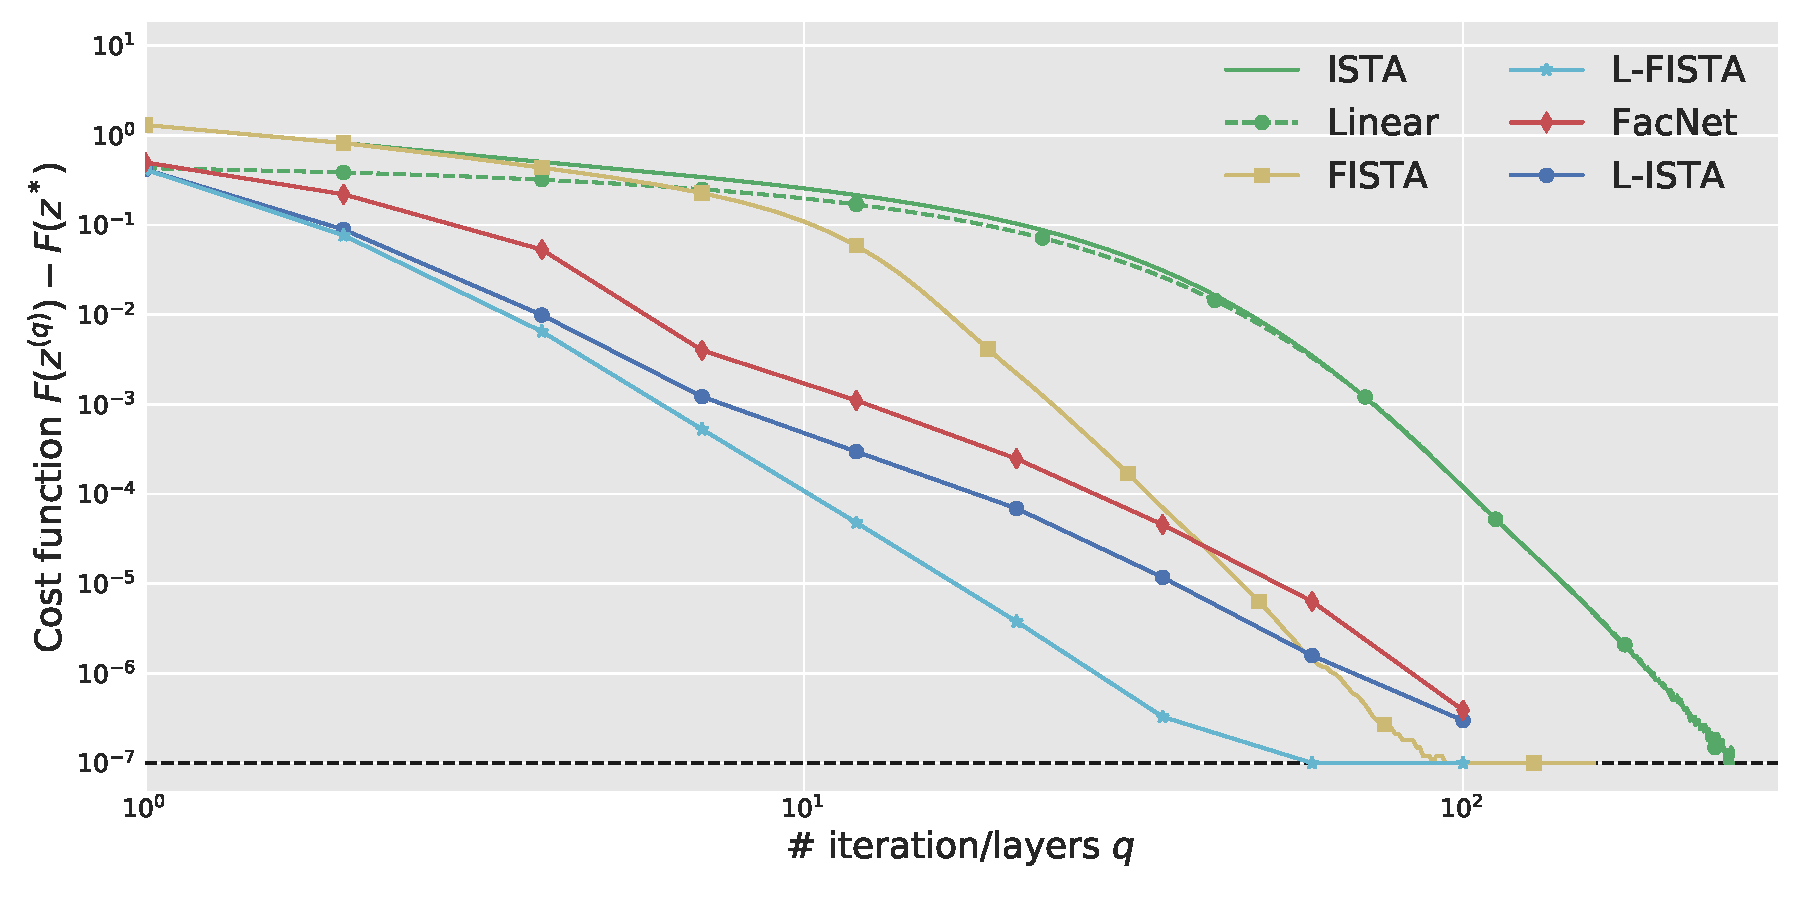
\includegraphics[width=.8\textwidth]{curve_sparse005_seaborn}\\
    Evolution of the cost function $F(z^{(q)}) - F(z^*)$ with the number of layers/iterations $q$ with a sparse model $\rho = {}^1/_{20}$.
\end{frame}

\begin{frame}[noframenumbering]{Artificial simulation}
\centering
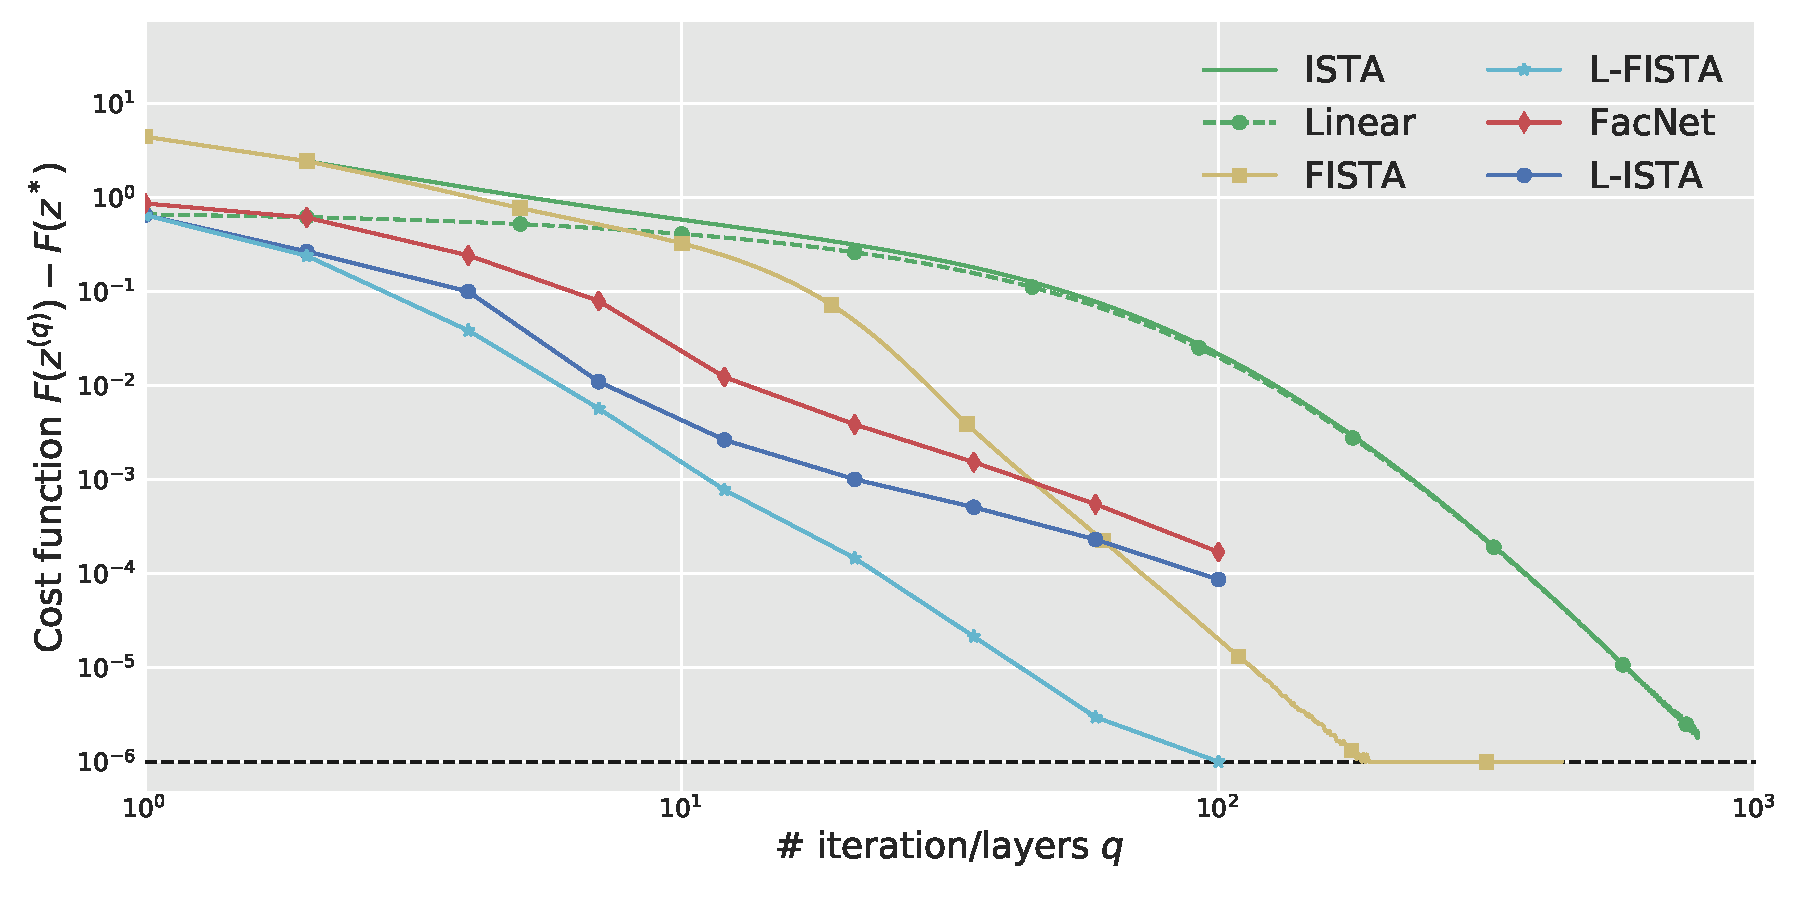
\includegraphics[width=.8\textwidth]{curve_sparse02_seaborn}\\
    Evolution of the cost function $F(z^{(q)}) - F(z^*)$ with the number of layers/iterations $q$ with a denser model $\rho = {}^1/_{4}$.
\end{frame}


\begin{frame}{Adversarial dictionary}

	\begin{columns}[T]
		\column{.35\textwidth}
		{\bf Adversarial dictionary:}\\
		$D = \begin{bmatrix} d_1 \dots d_K \end{bmatrix} \in \Rset^{K\times p}~,$ with 
		\[
			d_j = e^{-i \frac{2\pi j \zeta_q}{K}}
		\]
		for a random subset of frequencies $\left \{ \zeta_i \right \}_{i \le m}$ 
			
		\column{.65\textwidth}
		\includegraphics[width=\textwidth]{dictionary}
	\end{columns}
	\vskip2em
	\hskip2em $\Rightarrow$ Eigenvectors of $D$ are far from canonical basis.
\end{frame}


\begin{frame}[noframenumbering]{Adversarial dictionary}
\centering
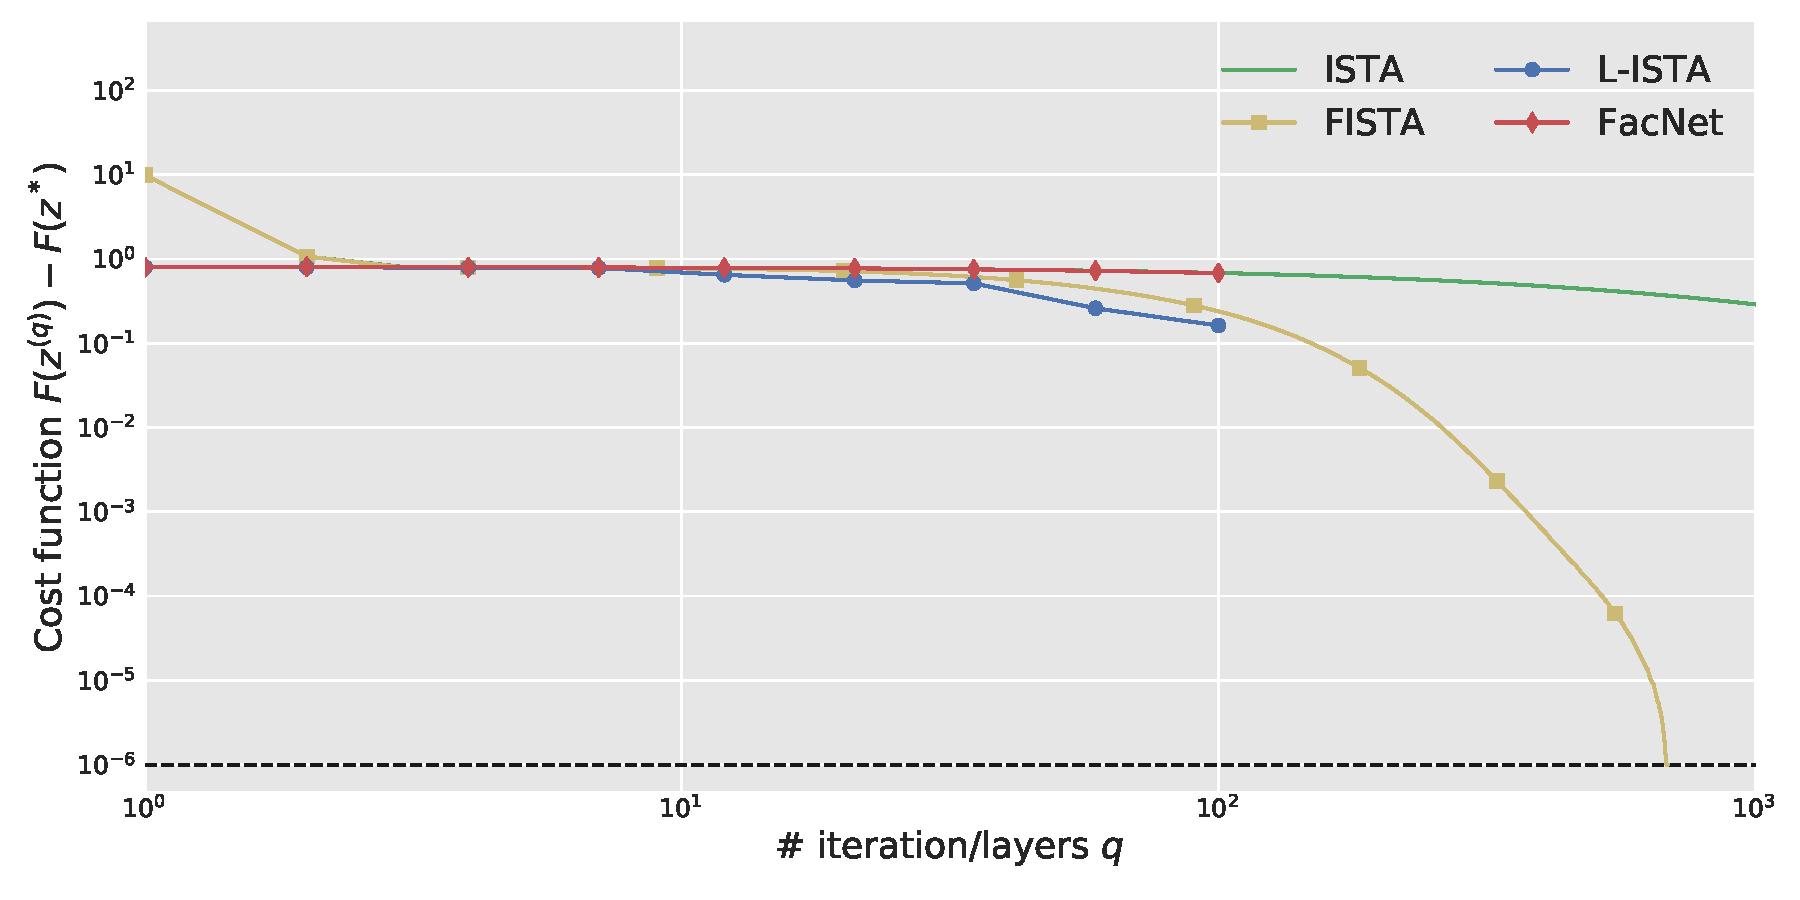
\includegraphics[width=.8\textwidth]{curve_adverse_seaborn}\\
    Evolution of the cost function $F(z^{(q)}) - F(z^*)$ with the number of layers/iterations k with n adversarial dictionary.
\end{frame}


\begin{frame}{Contribution}
\textbf{Contributions}
\begin{itemize}\itemsep.5em
	\item Non asymptotic acceleration of ISTA is possible based on the structure of $\pmb D$
	\item Sufficient analysis to explain LISTA acceleration,
	\item The dictionary structure seems necessary.
\end{itemize}

\vskip1.5em 
 \textbf{Future work:}
    \begin{itemize}\itemsep.5em
	    \item Improve the factorization formulation for direct optimization,
	    \item Second order analysis for generic dictionary,
	    \item Link to Sparse PCA.
    \end{itemize}
	
\end{frame}



\end{document}